%%%%%%%%%%%%%%%%%%%%%%%%%%%%%%%%%%%%%%%%%%%%%%%%%%%%%%%%%%%%%%%%%%%%%%%%%%%%%%%%
%% Plantilla de memoria en LaTeX para la ETSIT - Universidad Rey Juan Carlos
%%
%% Por Gregorio Robles <grex arroba gsyc.urjc.es>
%%     Grupo de Sistemas y Comunicaciones
%%     Escuela Técnica Superior de Ingenieros de Telecomunicación
%%     Universidad Rey Juan Carlos
%% (muchas ideas tomadas de Internet, colegas del GSyC, antiguos alumnos...
%%  etc. Muchas gracias a todos)
%%
%% La última versión de esta plantilla está siempre disponible en:
%%     https://github.com/gregoriorobles/plantilla-memoria
%%
%% Para obtener PDF, ejecuta en la shell:
%%   make
%% (las imágenes deben ir en PNG o JPG)

%%%%%%%%%%%%%%%%%%%%%%%%%%%%%%%%%%%%%%%%%%%%%%%%%%%%%%%%%%%%%%%%%%%%%%%%%%%%%%%%

\documentclass[a4paper, 12pt]{book}
%\usepackage[T1]{fontenc}

\usepackage[a4paper, left=2.5cm, right=2.5cm, top=3cm, bottom=3cm]{geometry}
\usepackage{times}
\usepackage[utf8]{inputenc}
\usepackage[spanish]{babel} % Comenta esta línea si tu memoria es en inglés
\usepackage{url}
%\usepackage[dvipdfm]{graphicx}
\usepackage{graphicx}
\usepackage{float}  %% H para posicionar figuras
\usepackage[nottoc, notlot, notlof, notindex]{tocbibind} %% Opciones de índice
\usepackage{latexsym}  %% Logo LaTeX

\title{Memoria del Proyecto}
\author{Vicente Giménez García}

\renewcommand{\baselinestretch}{1.5}  %% Interlineado

\begin{document}

\renewcommand{\refname}{Bibliografía}  %% Renombrando
\renewcommand{\appendixname}{Apéndice}

%%%%%%%%%%%%%%%%%%%%%%%%%%%%%%%%%%%%%%%%%%%%%%%%%%%%%%%%%%%%%%%%%%%%%%%%%%%%%%%%
% PORTADA

\begin{titlepage}
\begin{center}

\includegraphics[scale=0.8]{img/URJ_logo_Color_POS.png}

\vspace{1.75cm}

\Large
GRADO EN INGENIERÍA EN TECNOLOGÍAS DE TELECOMUNICACIÓN

\vspace{0.4cm}

\large
Curso Académico 2020/2021

\vspace{0.8cm}

Trabajo Fin de Grado

\vspace{2.5cm}

\LARGE
[TODO] TÍTULO DEL TRABAJO EN MAYÚSCULAS

\vspace{4cm}

\large
Autor : Vicente Giménez García \\
Tutor : Pedro de las Heras Quirós
\end{center}
\end{titlepage}

\newpage
\mbox{}
\thispagestyle{empty} % para que no se numere esta pagina


%%%%%%%%%%%%%%%%%%%%%%%%%%%%%%%%%%%%%%%%%%%%%%%%%%%%%%%%%%%%%%%%%%%%%%%%%%%%%%%%
%%%% Para firmar
\clearpage
\pagenumbering{gobble}
\chapter*{}

\vspace{-4cm}
\begin{center}
\LARGE
\textbf{Trabajo Fin de Grado}

\vspace{1cm}
\large
[TODO] Título del Trabajo con Letras Capitales para Sustantivos y Adjetivos

\vspace{1cm}
\large
\textbf{Autor :} Vicente Giménez García \\
\textbf{Tutor :} Pedro de las Heras Quirós

\end{center}

\vspace{1cm}
La defensa del presente Proyecto Fin de Carrera se realizó el día \qquad$\;\,$ de \qquad\qquad\qquad\qquad \newline de 2021, siendo calificada por el siguiente tribunal:


\vspace{0.5cm}
\textbf{Presidente:}

\vspace{1.2cm}
\textbf{Secretario:}

\vspace{1.2cm}
\textbf{Vocal:}


\vspace{1.2cm}
y habiendo obtenido la siguiente calificación:

\vspace{1cm}
\textbf{Calificación:}


\vspace{1cm}
\begin{flushright}
Fuenlabrada, a \qquad$\;\,$ de \qquad\qquad\qquad\qquad de 202X
\end{flushright}

%%%%%%%%%%%%%%%%%%%%%%%%%%%%%%%%%%%%%%%%%%%%%%%%%%%%%%%%%%%%%%%%%%%%%%%%%%%%%%%%
%%%% Dedicatoria

\chapter*{}
\pagenumbering{Roman} % para comenzar la numeracion de paginas en numeros romanos
\begin{flushright}
\textit{[TODO] Dedicado a \\
mi familia / mi abuelo / mi abuela}
\end{flushright}

%%%%%%%%%%%%%%%%%%%%%%%%%%%%%%%%%%%%%%%%%%%%%%%%%%%%%%%%%%%%%%%%%%%%%%%%%%%%%%%%
%%%% Agradecimientos

\chapter*{Agradecimientos}
%\addcontentsline{toc}{chapter}{Agradecimientos} % si queremos que aparezca en el índice
\markboth{AGRADECIMIENTOS}{AGRADECIMIENTOS} % encabezado 

[TODO] Aquí vienen los agradecimientos\ldots Aunque está bien acordarse de la pareja, no hay que olvidarse de dar las gracias a tu madre, que aunque a veces no lo parezca disfrutará tanto de tus logros como tú\ldots 
Además, la pareja quizás no sea para siempre, pero tu madre sí.

%%%%%%%%%%%%%%%%%%%%%%%%%%%%%%%%%%%%%%%%%%%%%%%%%%%%%%%%%%%%%%%%%%%%%%%%%%%%%%%%
%%%% Resumen

\chapter*{Resumen}
%\addcontentsline{toc}{chapter}{Resumen} % si queremos que aparezca en el índice
\markboth{RESUMEN}{RESUMEN} % encabezado

Una de las dificultades a las que se enfrentan los alumnos en período de prácticas empresariales o recién egresados de la universidad 
es el desconocimiento de qué salario podría considerarse justo para un determinado puesto ante una oferta de trabajo.

A esta dificultad se añade el hecho de que muichos trabajadores consideran hablar de su sueldo un tema tabú,
lo que complica a aquellos alumnos que buscan trabajo la tarea de recabar información acerca de qué rango salarial es el adecuado para una determinada actividad.

Además, concretamente en el ámbito de las tecnologías de la información y la comunicación, el gran abanico de sectores, profesiones, técnicas, lenguajes, etcétera, 
hace que resulte realmente complejo para una persona con poca experiencia evaluar si una oferta de trabajo es interesante desde un punto de vista económico.

Con el objetivo de facilitar a los alumnos esta tarea de entendimiento del mercado, este proyecto pretende plantear una solución sencilla y eficaz en forma de aplicación 
web que permite buscar y compartir información laboral de primera mano a través de las experiencias laborales de los usuarios que participan en la plataforma.

Esta aplicación enfatiza en el intercambio de información laboral entre dos usuarios como fuente información, permitiendo en todos los casos que estos compartan únicamente los datos que deseen mostrar acerca de una experiencia laboral propia, 
incluida su identidad en caso de que prefieran ofrecer sus referencias de forma anónima.

Este proyecto se compone de un servidor que expone su funcionalidad a través de un API REST, desarrollado con la tecnología Spring Boot y una aplicación de navagdor en el lado del cliente desarrollada en React que consume los recursos expuestos en dicha API. 
Todo el sistema es accesible a través de autenticación de los usuarios en la plataforma de Github, lo que permite a la mayoría de los alumnos de grados relacionados con las TIC poder hacer uso de la aplicación sin tener que hacer un registro adicional.

%%%%%%%%%%%%%%%%%%%%%%%%%%%%%%%%%%%%%%%%%%%%%%%%%%%%%%%%%%%%%%%%%%%%%%%%%%%%%%%%
%%%%%%%%%%%%%%%%%%%%%%%%%%%%%%%%%%%%%%%%%%%%%%%%%%%%%%%%%%%%%%%%%%%%%%%%%%%%%%%%
% ÍNDICES %
%%%%%%%%%%%%%%%%%%%%%%%%%%%%%%%%%%%%%%%%%%%%%%%%%%%%%%%%%%%%%%%%%%%%%%%%%%%%%%%%.

%%%% Índice de contenidos
\tableofcontents 
%%%% Índice de figuras
\cleardoublepage
%\addcontentsline{toc}{chapter}{Lista de figuras} % para que aparezca en el indice de contenidos
\listoffigures % indice de figuras
%%%% Índice de tablas
%\cleardoublepage
%\addcontentsline{toc}{chapter}{Lista de tablas} % para que aparezca en el indice de contenidos
%\listoftables % indice de tablas


%%%%%%%%%%%%%%%%%%%%%%%%%%%%%%%%%%%%%%%%%%%%%%%%%%%%%%%%%%%%%%%%%%%%%%%%%%%%%%%%
%%%%%%%%%%%%%%%%%%%%%%%%%%%%%%%%%%%%%%%%%%%%%%%%%%%%%%%%%%%%%%%%%%%%%%%%%%%%%%%%
% INTRODUCCIÓN %
%%%%%%%%%%%%%%%%%%%%%%%%%%%%%%%%%%%%%%%%%%%%%%%%%%%%%%%%%%%%%%%%%%%%%%%%%%%%%%%%

\cleardoublepage
\chapter{Introducción}
\label{sec:intro} % etiqueta para poder referenciar luego en el texto con ~\ref{sec:intro}
\pagenumbering{arabic} % para empezar la numeración de página con números

Este Trabajo fin de Grado consiste en una aplicación web desarrollada en una arquitectura cliente-servidor que tiene el próposito de permitir a los usuarios crear, modificar y eliminar sus experiencias laborales con un nivel de privacidad establecido por el propio usuario
de forma que sean accesibles mediante una búsqueda por el resto de los usuarios, que pueden solicitar información privada acerca de estas a cambio de ofrecer la suya propia. 
En esta arquitectura, el cliente es una aplicación JavaScript ejecutable en el navegador, 
y el servidor es un servidor de aplicaciones Java EE cuyos recursos son accesibles por el cliente a través de un API REST. Además, la aplicación utiliza GitHub como proveedor de autenticación para los usuarios. 
A continuación se procederá a describir tanto cada una de las partes de la aplicación como las tecnologías utilizadas y las herramientas empleadas para su desarrollo.

\section{Definición de experiencia laboral}
\label{sec:intro_workexperiencedefinition}
En el contexto de este Trabajo Fin de Grado, se considerará una experiencia laboral de un usuario al conjunto de datos formados por:

\begin{itemize}
  \item La empresa donde transcurrió la experiencia laboral.
  \item El puesto que se desempeñó dentro de la empresa.
  \item El conjunto de tecnologías de las que el usuario hizo uso durante el ejercicio de su actividad.
  \item El periodo durante el que se ejerció la actividad en la empresa, con fecha de inicio y fecha de fin en el caso de experiencias pasadas.
  \item El salario bruto anual representativo que percibió el usuario durante el periodo laboral.
\end{itemize}

\section{Privacidad}
\label{sec:intro_privacity}
Para cada una de las experiencias que un usuario agregue al sistema, este podrá decidir todo momento la visibilidad que tendrá cada uno de los campos de la definición de experiencia laboral para el resto de usuarios, siendo posible que un campo sea público, lo que lo hará visible para la totalidad de los usuarios, o privado, en cuyo caso solo será visible para aquellos usuarios que mediante  una solicitud de información hayan obtenido permiso para visualizar dicho campo.

Adicionalmente, los usuarios podrán elegir dentro de sus experiencias, cuales de ellas serán vinculadas a su perfil. Aquellas que no sean vinculadas aparecerán vinculadas a un usuario anónimo en las búsquedas que hagan el resto de usuarios, siendo imposible reconocer a quién pertenecen.

\section{Solicitud de información a otros usuarios}
\label{sec:intro_inforequest}
Dada una experiencia laboral determinada, en la que uno o varios de los campos hayan sido declarados como privados por su poseedor, es posible para otros usuarios solicitar revelar estos campos. 
Para esto el usuario interesado envía una solicitud de información en la que indica cuales de estos campos quiere que le sean revelados, y opcionalmente, ofrece revelar campos privados de alguna de sus experiencias a cambio al usuario receptor de la solicitud.
En este momento se establece una negociación entre ambos usuarios, en el que cada uno de ellos, por turnos, puede modificar lo que ofrece y solicita revelar. Esta negociación finalizada cuando el usuario al que corresponde realizar el siguiente paso de la negociación acepta el intercambio de datos, o en el momento en el que uno de ambos usuarios deniega la solicitud.


\section{Servidor de aplicaciones}
\label{sec:intro_applicationserver}

Es la pieza de software que no se ejecuta en el navegador si no que es invocada desde este vía conexión HTTP. 
Su cometido en la aplicación es el de exponer recursos que ofrecen la información de los usuarios, es decir, sus experiencias laborales y solicitudes de manera controlada basada en la identidad de los usuarios. 
Para ello antes de ofrecer información al lado cliente comprueba la identidad del usuario que la solicita para aplicarle las reglas de visibilidad y presentar únicamente la información que, 
o bien es pública, o bien pertenece al solicitante, o bien tanto el solicitante como el propietario han accedido a compartir. Abajo se describirán los puntos principales relacionados con el servidor de aplicaciones.

\subsection{Lenguaje y plataforma}
\label{subsec:intro_applicationserver_languageandplatform}

El lenguaje elegido para el desarrollo del servidor es Java. Java es un lenguaje de programación orientada objetos desarrollado por la compañía Sun Microsystems. 
Una de sus particularidades más importantes es la de poder ejecutarse en la máquina virtual de Java (JVM) que puede ser instalada en la gran mayoría de sistemas operativos, 
lo que proporciona a este lenguaje gran portabilidad entre distintas plataformas. La versión concreta de Java que se utilizó para el desarrollo fue la 11, que entre otras características da Java soporte para la programación funcional.

El framework Java utilizado para la creación del servidor fue Spring, un framework Open Source que facilita el desarrollo de aplicaciones Java Enterprise Edition, que es a su vez una plataforma, parte de la plataforma Java que permite el desarrollo de aplicaciones servidor. 
Spring Framework provee una serie de características y librerías que ayudan al programador a centrarse en el desarrollo de la lógica que quiere implementar en su aplicación, abstrayéndose de conceptos de infraestructura que complican el desarrollo de servidores.
 Para esta aplicación se utilizó concretamente la tecnología Spring Boot que además reduce la cantidad de configuración necesaria para funcionamiento de una aplicación Spring.

\subsection{Comunicación con el cliente}
\label{subsec:intro_applicationserver_communicationwithclient}

Para permitir a la parte cliente del navegador acceder la información laboral que reside en el servidor, la aplicación servidor expone un API REST. 
Un API REST es una interfaz accesible de forma remota vía protocolo HTTP donde la información se representa en forma de recurso, siendo estos recursos identificadores de los conceptos y entidades que alberga el servidor, que en el caso de este Trabajo Fin de Grado son las experiencias laborales y las solicitudes de información. 
En un API REST estos recursos son operables utilizando los propios métodos HTTP, a los que el estilo REST provee de semántica, interpretándose los verbos HTTP como operaciones de escritura, lectura, borrado y modificación. De esta forma un cliente web puede en este caso crear, borrar, leer y modificar experiencias laborales y solicitudes dentro del servidor enviando mensajes HTTP.

\subsection{Base de datos}
\label{subsec:intro_applicationserver_database}

Para almacenar las experiencias laborales de los usuarios y solicitudes, el servidor hace uso de una base de datos relacional (SQL), concretamente H2, que es un motor de bases de datos Open Source cuyas características principales son estar implementado en Java, 
lo que simplifica en muchos casos la integración con aplicaciones Java, y el poder levantarse en memoria o en modo embebido, de forma que sus datos se almacenan en ficheros, lo que facilita la base de desarrollo, evitando al programador tener que instalar y configurar una base de datos completa. 
El dialecto SQL que utiliza H2 es altamente compatible con el resto de dialectos de SQL, lo que a futuro permite hacer uso de otro distribuidor distinto de base de datos sin realizar grandes modificaciones.

Como librería para realizar operaciones de base de datos desde el servidor se ha hecho uso de MyBatis, una herramienta de persistencia de Java que permite definir sentencias SQL en archivos XML que pueden ser invocadas desde el código y que integra fácilmente con Spring Framework.

La herramienta para definir la estructura de la base de datos es Flyway, una tecnología que permite llevar un versionado de la base de datos mediante una lista de scripts SQL, uno por versión. Estos scripts se ejecutan secuencialmente, por lo que cada script debe escribirse como una modificación del estado de la estructura de base de datos que dejó el script anterior. 
De esta manera Flyway es capaz de llevar un registro de que modificaciones se hicieron en anteriores desarrollos sobre el proyecto, para ejecutar solo los nuevos scripts, es decir, los últimos cambios, no teniendo que generar una estructura nueva en cada modificación, lo que facilita la modificación de la base de datos una vez la aplicación está en producción, 
sin la pérdida de datos que supondría eliminar toda la estructura SQL y volverla a crear en cada modificación.


\section{Aplicación web}
\label{sec:intro_webapplication}

Es la aplicación que se ejecuta en el navegador web del usuario. Su función es la de ofrecer una interfaz amigable e intuitiva al usuario para permitirle operar sobre sus recursos en el servidor y realizar consultas de datos. 
En el caso concreto de este Trabajo Fin de Grado, la aplicación web ofrece una interfaz para que el usuario pueda crear, modificar e eliminar sus experiencias laborales, realizar búsquedas de experiencias laborales mediante filtros 
y crear solicitudes de datos confidenciales a otros usuarios desde su navegador, mediante una interfaz gráfica.

\subsection{Lenguaje y librerías}
\label{subsec:intro_webapplication_languageandlibraries}

El lenguaje utilizado para desarrollar la lógica en esta parte fue JavaScript. Este es un lenguaje interpretado orientado a objetos, que se ejecuta en los navegadores y permite modificar el documento HTML que visualiza el usuario, solicitar datos remotos a un servidor y almacenar datos en el propio navegador entre otras funciones.

La librería utilizada para el desarrollo de la aplicación fue React, una librería que facilita el desarrollo de aplicaciones JavaScript de una sola página, cuya característica principal es la facilidad que aporta a la hora de desarrollar componentes web, es decir, 
componentes reutilizables en la aplicación, que se pueden invocar múltiples veces en el código mediante una etiqueta y atributos que actúan como entrada de información en el componente, y que tienen su propia estructura interna, comportamiento y estilo. 
Para esto React hace uso de archivos JavaScript con una extensión específica, JSX, que permiten referenciar HTML directamente desde el código JavaScript como si se tratara de un tipo de dato adicional a los que el JavaScript nativo soporta. 
Debido al uso de esta librería, la presencia de archivos HTML en la aplicación web es mínima, limitándose a un único archivo prácticamente vacío cuya función es referenciar los recursos necesarios para la ejecución de la aplicación.


\subsection{Estilo}
\label{subsec:intro_webapplication_style}

Para agregar estilos a la interfaz gráfica y hacer la aplicación visualmente más atractiva se ha hecho uso de la librería Bootstrap. Bootstrap provee una serie de estilos CSS predefinidos y fácilmente utilizables sobre los elementos HTML de la aplicación en forma de clases HTML.

\section{Autenticación}
\label{sec:intro_authentication}

Con el objetivo de facilitar a los usuarios el ingreso en la aplicación, esta se ha integrado con la plataforma GitHub, haciendo uso de ella como proveedora de autenticación e identidad. De esta manera, los usuarios que ya están registrados en GitHub, como suele ser el caso de los alumnos de carreras relacionadas con las TIC, pueden utilizar sus credenciales de GitHub para acceder a la aplicación. Estas credenciales se envían directamente a GitHub, por lo que no pasan directamente por la aplicación de este Trabajo Fin de Grado, de forma que en ningún momento se pone en riesgo la privacidad del usuario.

Para lograr esto se ha hecho uso del módulo Spring Social, que facilita la comunicación con GitHub vía el estándar OAuth2, una forma de integrar aplicaciones con plataformas que ofrecen parte de los datos de sus usuarios sin vulnerar su privacidad, extendiendo la sesión de estos usuarios a aplicaciones de terceros.


\section{Herramientas}
\label{sec:intro_tools}
A continuación se exponen brevemente algunas de las principales herramientas que se utilizaron para el desarrollo de la aplicación.

\subsection{IntelliJ IDEA}
\label{subsec:intro_tools_intellij}
IntelliJ IDEA es un entorno de desarrollo integrado desarrollado por la compañía JetBrains. Tiene soporte para el lengauje Java, facilita las tareas de escritura del código, permite ejecutar y depurar aplicaciones y pruebas, integra con varias herramientas de gestión de dependencias y control de versiones, entre otras características. Se eligió este IDE para hacer el desarrollo del servidor de aplicaciones.

\subsection{Visual Studio Code}
\label{subsec:intro_tools_vsc}
Visual Studio Code es un editor de código fuente con gran soporte para JavaScript. Permite ejecutar y depurar aplicaciones y pruebas, integra con gestores de dependencias y control de versiones. Se eligió este editor para el desarrollo de la aplicación web en React.

\subsection{Maven}
\label{subsec:intro_tools_maven}
Maven es una herramienta de gestión de proyectos de software desarrollada por Apache Software Foundation. Permite de forma declarativa gestionar todas las dependencias de un proyecto Java, es decir, referenciar los módulos que contienen las librerías sobre las que se construye el proyecto para poder descargarlos automáticamente del repositorio central de Maven
durante la construcción de la aplicación. También permite la ejecución de plugins que facilitan tareas de desarrollo como construcción, ejecución de pruebas, empaquetado, instalación, etcétera. Se utilizó para la gestión de dependecias del servidor de aplicaciones.

\subsection{NPM}
\label{subsec:intro_tools_npm}
NPM es el sistema de gestión de paquetes para el lenguaje JavaScript. De forma similar a Maven permite gestionar las dependencias de una aplicación web JavaScript declarándolas en un fichero y automatizando de esta forma su descarga. Se utilizó para la gestión de dependencias de la aplicación web.


\subsection{Git}
\label{subsec:intro_tools_git}
Git es un sistema de control de versiones distribuido y de código abierto. Permite mantener un histórico de los cambios del proyecto de forma remota (en este caso en Github) y una copia de estos de forma local. Además permite mantener distintas ramas de desarollo en paralelo, esta característica facilita el desarollo de distintas funcionalidades del software en paralelo, ya sea por uno o varios desarrolladores, siendo posible mezclar estas distintas ramas después con la versión final, gestionando mediante el sistema Git las diferencias y conflictos entre los cambios en el código.

\section{Estructura de la memoria}
\label{sec:intro_memorystructure}
[TODO]


%%%%%%%%%%%%%%%%%%%%%%%%%%%%%%%%%%%%%%%%%%%%%%%%%%%%%%%%%%%%%%%%%%%%%%%%%%%%%%%%
%%%%%%%%%%%%%%%%%%%%%%%%%%%%%%%%%%%%%%%%%%%%%%%%%%%%%%%%%%%%%%%%%%%%%%%%%%%%%%%%
% OBJETIVOS %
%%%%%%%%%%%%%%%%%%%%%%%%%%%%%%%%%%%%%%%%%%%%%%%%%%%%%%%%%%%%%%%%%%%%%%%%%%%%%%%%

\cleardoublepage % empezamos en página impar
\chapter{Objetivos} % título del capítulo (se muestra)
\label{chap:targets} % identificador del capítulo (no se muestra, es para poder referenciarlo)

\section{Objetivo general} % título de sección (se muestra)
\label{sec:targets_generaltarget} % identificador de sección (no se muestra, es para poder referenciarla)

El objetivo de este Trabajo Fin de Grado es desarrollar una aplicación que permita a estudiantes y trabajadores del sector de las tecnologías de la información y la comunicación evaluar cual es el rango salarial justo para una determinada profesión u oferta de trabajo teniendo en cuenta la empresa donde se realizará la labor, el cargo y las tecnologías relacionadas con el puesto.


\section{Objetivos específicos}
\label{sec:target_specifictargets}

Los objetivos específicos de este Trabajo Fin de Grado son:

\begin{enumerate}
  \item Proporcionar a los usuarios del sector TIC un método para ingresar fácilmente en la aplicación sin necesidad de registrarse, mediante un proveedor de autenticación externo.
  \item Permitir a los usuarios añadir, modificar y eliminar sus experiencias laborales en el sistema a través de la aplicación.
  \item Dar opción a los usuarios para que estas experiencias laborales no se vinculen con su perfil, de manera que sean visibles a otros usuarios sin conocer la identidad de aquel al que pertenecen.
  \item Permitir a los usuarios declarar parte o todos los datos relacionados con una de sus experiencias laborales como privados de forma que solo sean visibles para otros usuarios mediante un acuerdo con el poseedor.
  \item Proporcionar a los usuarios un mecanismo de búsqueda de experiencias laborales de otros usuarios.
  \item Permitir filtrar estas búsquedas por puesto, empresa, tecnologías, salario mínimo y máximo y fecha de inicio mínima y máxima.
  \item Dar opción a los usuarios de solicitar información privada de una experiencia ajena mediante el envío de un solcitud a su propietario, pudiendo ofrecer el solicitante datos privados de alguna de sus propias experiencias a cambio.
  \item Ofrecer un mecanismo para que los usuarios puedan renegociar por turnos que datos mostrarán y solicitan sobre una determinada solicitud.
  \item Ofrecer un mecanismo para poder aceptar o denegar solicitudes de datos privados.
  \item Permitir ver a los usuarios el histórico de los estados por los que ha pasado la negociación de una solcitud en vuelo o finalizada.
  \item En caso de que una solicitud de datos sea aceptada, permitir a los usuarios visualizar los datos privados ahora visibles como resultado de la negociación.
\end{enumerate}

\section{Planificación temporal}
\label{sec:planificacion-temporal}

[TODO]
A mí me gusta que aquí pongáis una descripción de lo que os ha llevado realizar el trabajo.
Hay gente que añade un diagrama de GANTT.
Lo importante es que quede claro cuánto tiempo llevas (tiempo natural, p.ej., 6 meses) y a qué nivel de esfuerzo (p.ej., principalmente los fines de semana).


\subsection{Estilo}
\label{subsec:estilo}
[TODO][REMOVE]

Recomiendo leer los consejos prácticos sobre escribir documentos científicos en \LaTeX \ de Diomidis Spinellis\footnote{\url{https://github.com/dspinellis/latex-advice}}.

Lee sobre el uso de las comas\footnote{\url{http://narrativabreve.com/2015/02/opiniones-de-un-corrector-de-estilo-11-recetas-para-escribir-correctamente-la-coma.html}}. 
Las comas en español no se ponen al tuntún.
Y nunca, nunca entre el sujeto y el predicado (p.ej. en ``Yo, hago el TFG'' sobre la coma).
La coma no debe separar el sujeto del predicado en una oración, pues se cortaría la secuencia natural del discurso.
No se considera apropiado el uso de la llamada coma respiratoria o \emph{coma criminal}.
Solamente se suele escribir una coma para marcar el lugar que queda cuando omitimos el verbo de una oración, pero es un caso que se da de manera muy infrecuente al escribir un texto científico (p.ej. ``El Real Madrid, campeón de Europa'').

A continuación, viene una figura, la Figura~\ref{figura:foro_hilos}. 
Observarás que el texto dentro de la referencia es el identificador de la figura (que se corresponden con el ``label'' dentro de la misma). 
También habrás tomado nota de cómo se ponen las ``comillas dobles'' para que se muestren correctamente. 
Nota que hay unas comillas de inicio (``) y otras de cierre (''), y que son diferentes.
Volviendo a las referencias, nota que al compilar, la primera vez se crea un diccionario con las referencias, y en la segunda compilación se ``rellenan'' estas referencias. 
Por eso hay que compilar dos veces tu memoria.
Si no, no se crearán las referencias.

 \begin{figure}
    \centering
    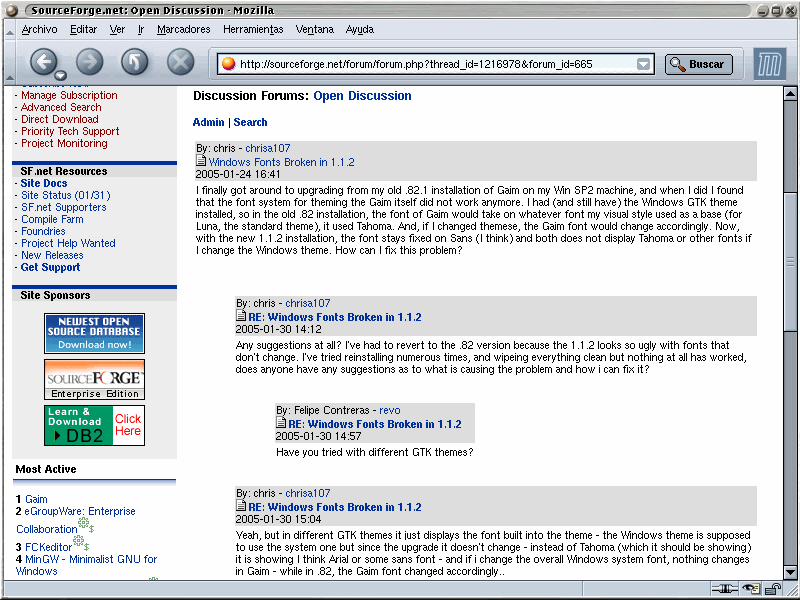
\includegraphics[bb=0 0 800 600, width=12cm, keepaspectratio]{img/foro1}
    \caption{Página con enlaces a hilos}
    \label{figura:foro_hilos}
 \end{figure}

A continuación un bloque ``verbatim'', que se utiliza para mostrar texto tal cual.
Se puede utilizar para ofrecer el contenido de correos electrónicos, código, entre otras cosas.

{\footnotesize
\begin{verbatim}
    From gaurav at gold-solutions.co.uk  Fri Jan 14 14:51:11 2005
    From: gaurav at gold-solutions.co.uk (gaurav_gold)
    Date: Fri Jan 14 19:25:51 2005
    Subject: [Mailman-Users] mailman issues
    Message-ID: <003c01c4fa40$1d99b4c0$94592252@gaurav7klgnyif>

    Dear Sir/Madam,
    How can people reply to the mailing list?  How do i turn off
    this feature? How can i also enable a feature where if someone
    replies the newsletter the email gets deleted?
    Thanks

    From msapiro at value.net  Fri Jan 14 19:48:51 2005
    From: msapiro at value.net (Mark Sapiro)
    Date: Fri Jan 14 19:49:04 2005
    Subject: [Mailman-Users] mailman issues
    In-Reply-To: <003c01c4fa40$1d99b4c0$94592252@gaurav7klgnyif>
    Message-ID: <PC173020050114104851057801b04d55@msapiro>

    gaurav_gold wrote:
    >How can people reply to the mailing list?  How do i turn off
    this feature? How can i also enable a feature where if someone
    replies the newsletter the email gets deleted?

    See the FAQ
    >Mailman FAQ: http://www.python.org/cgi-bin/faqw-mm.py
    article 3.11
\end{verbatim}
}

\section{Estructura de la memoria}
\label{sec:estructura}

En esta sección se debería introducir la esctura de la memoria. 

Así:

\begin{itemize}
  \item En el primer capítulo se hace una intro al proyecto.
  
  \item En el capítulo~\ref{chap:objetivos} (ojo, otra referencia automática) se muestran los objetivos del proyecto.
  
  \item A continuación se presenta el estado del arte en el capítulo~\ref{chap:estado}.
  
  \item \ldots
\end{itemize}




%%%%%%%%%%%%%%%%%%%%%%%%%%%%%%%%%%%%%%%%%%%%%%%%%%%%%%%%%%%%%%%%%%%%%%%%%%%%%%%%
%%%%%%%%%%%%%%%%%%%%%%%%%%%%%%%%%%%%%%%%%%%%%%%%%%%%%%%%%%%%%%%%%%%%%%%%%%%%%%%%
% ESTADO DEL ARTE %
%%%%%%%%%%%%%%%%%%%%%%%%%%%%%%%%%%%%%%%%%%%%%%%%%%%%%%%%%%%%%%%%%%%%%%%%%%%%%%%%

\cleardoublepage
\chapter{Estado del arte}
\label{chap:estado}

Descripción de las tecnologías que utilizas en tu trabajo. 
Con dos o tres párrafos por cada tecnología, vale. 
Se supone que aquí viene todo lo que no has hecho tú.

Puedes citar libros, como el de Bonabeau et al., sobre procesos estigmérgicos~\cite{bonabeau:_swarm}. 
Me encantan los procesos estigmérgicos.
Deberías leer más sobre ellos.
Pero quizás no ahora, que tenemos que terminar la memoria para sacarnos por fin el título.
Nota que el \~ \ añade un espacio en blanco, pero no deja que exista un salto de línea. 
Imprescindible ponerlo para las citas.

Citar es importantísimo en textos científico-técnicos. 
Porque no partimos de cero.
Es más, partir de cero es de tontos; lo suyo es aprovecharse de lo ya existente para construir encima y hacer cosas más sofisticadas.
¿Dónde puedo encontrar textos científicos que referenciar?
Un buen sitio es Google Scholar\footnote{\url{http://scholar.google.com}}.
Por ejemplo, si buscas por ``stigmergy libre software'' para encontrar trabajo sobre software libre y el concepto de \emph{estigmergia} (¿te he comentado que me gusta el concepto de estigmergia ya?), encontrarás un artículo que escribí hace tiempo cuyo título es ``Self-organized development in libre software: a model based on the stigmergy concept''.
Si pulsas sobre las comillas dobles (entre la estrella y el ``citado por ...'', justo debajo del extracto del resumen del artículo, te saldrá una ventana emergente con cómo citar.
Abajo a la derecha, aparece un enlace BibTeX.
Púlsalo y encontrarás la referencia en formato BibTeX, tal que así:

{\footnotesize
\begin{verbatim}
@inproceedings{robles2005self,
  title={Self-organized development in libre software:
         a model based on the stigmergy concept},
  author={Robles, Gregorio and Merelo, Juan Juli\'an 
          and Gonz\'alez-Barahona, Jes\'us M.},
  booktitle={ProSim'05},
  year={2005}
}
\end{verbatim}
}

Copia el texto en BibTeX y pégalo en el fichero \texttt{memoria.bib}, que es donde están las referencias bibliográficas.
Para incluir la referencia en el texto de la memoria, deberás citarlo, como hemos hecho antes con~\cite{bonabeau:_swarm}, lo que pasa es que en vez de el identificador de la cita anterior (bonabeau:\_swarm), tendrás que poner el nuevo (robles2005self).
Compila el fichero \texttt{memoria.tex} (\texttt{pdflatex memoria.tex}), añade la bibliografía (\texttt{bibtex memoria.aux}) y vuelve a compilar \texttt{memoria.tex} (\texttt{pdflatex memoria.tex})\ldots y \emph{voilà} ¡tenemos una nueva cita~\cite{robles2005self}!

También existe la posibilidad de poner notas al pie de página, por ejemplo, una para indicarte que visite la página del GSyC\footnote{\url{http://gsyc.es}}.



\section{Sección 1} 
\label{sec:seccion1}

Hemos hablado de cómo incluir figuras.
Pero no hemos dicho nada de tablas.
A mí me gustan las tablas.
Mucho.
Aquí un ejemplo de tabla, la Tabla~\ref{tabla:ejemplo} (siento ser pesado, pero nota cómo he puesto la referencia).

\begin{table}
 \begin{center}
  \begin{tabular}{ | l | c | r |} % tenemos tres colummnas, la primera alineada a la izquierda (l), la segunda al centro (c) y la tercera a la derecha (r). El | indica que entre las columnas habrá una línea separadora.
    \hline
    Uno & 2 & 3 \\ \hline % el hline nos da una línea vertical
    Cuatro & 5 & 6 \\ \hline
    Siete & 8 & 9 \\
    \hline
  \end{tabular}
  \label{tabla:ejemplo}
  \caption{Ejemplo de tabla. Aquí viene una pequeña descripción (el \emph{caption}) del contenido de la tabla. Si la tabla no es autoexplicativa, siempre viene bien aclararla aquí.}
 \end{center}
\end{table}



%%%%%%%%%%%%%%%%%%%%%%%%%%%%%%%%%%%%%%%%%%%%%%%%%%%%%%%%%%%%%%%%%%%%%%%%%%%%%%%%
%%%%%%%%%%%%%%%%%%%%%%%%%%%%%%%%%%%%%%%%%%%%%%%%%%%%%%%%%%%%%%%%%%%%%%%%%%%%%%%%
% DISEÑO E IMPLEMENTACIÓN %
%%%%%%%%%%%%%%%%%%%%%%%%%%%%%%%%%%%%%%%%%%%%%%%%%%%%%%%%%%%%%%%%%%%%%%%%%%%%%%%%

\cleardoublepage
\chapter{Diseño e implementación}

En este capítulo de describirá con detalle técnico el diseño e implementación de la aplicación completa desarrollada para este Trabajo Fin de Grado.

\section{Arquitectura general} 
\label{sec:architecture}

Como se indicó anteriormente el sitema está compuesto por una aplicación web de navegador desarrollada en React y un servidor web desarrollado en Spring Boot. 

La aplicación web consiste en una única página web compuesta de componentes web de primer nivel, que denominamos vistas, y que contienen a su vez por componentes web de segundo nivel.
Los componentes de primer nivel, llamados vistas, renderizan pantallas completas de la aplicación de una sola página, y tienen cada uno asociada una ruta de navegador.
Los componentes de segundo nivel, renderizan elementos web reutilizables dentro de las distintas vistas, como entradas de texto, tarjetas, etcétera. En algunos casos un componente de segundo nivel puede hacer uso de otros componentes de segundo nivel para extender su funcionalidad.
Además, la aplicación tiene un componente web de enrutado que permite navegar entre las distintas vistas, implementado con la tecnología React Router, que consiste en una barra de navegación horizontal en la parte superior de la pantalla.

El servidor fue desarrollado siguiendo una arquitectura hexagonal, también denominada patrón de puertos y adaptadores. Esta arquitectura presenta una serie de capas concéntricas con responsabilidades definidas.
Podemos definir la aplicación de esta arquitectura al sistema implementado para este Trabajo Fin de Grado a partir de los elementos que la componen, más interno a más externo:

\begin{itemize}
\item Modelo de dominio: Compuesto por las clases que representan los conceptos con los que nuestro sistema opera, en este caso el dominio corresponde principalmente con los conceptos de experiencia laboral y negociación (también llamada solicitud de información). 
El modelo de dominio no debe tener dependencia con ninguna otra capa de la aplicación.
Aunque posteriormente se describirá en mayor detalle, podemos distinguir las clases del modelo de dominio en dos tipos distintos:

	\begin{itemize}
	 \item Entidades: son aquellas que son susceptibles de ser identificadas mediante un identificador único y que tienen ciclo de vida, es decir, evolucionan a lo largo del tiempo a través de las operaciones que los usuarios realizan sobre ellas. 
	Podemos decir que dos entidades con igual información no son la misma entidad si difieren en su identificador único.
	Las entidades no son meras estructuras de datos anémicas, sino que continen la lógica necesaria para construirse, para cambiar de estado, para validar la información de la que se componen o la que transitan y para interoperar con otras entidades.
	Además son las propias entidades las que generan proyecciones de si mismas omitiendo datos en caso de que el usuario que las accede no tenga visibilidad sobre estos datos, por lo que son las encargadas de aplicar los criterios de privacidad.
	Desde este punto de vista podemos afirmar que las entidades contienen la lógica de negocio de la aplicación.
	Las entidades de este sistema son las experiencias laborales y las negociaciones.

	\item Objetos de valor: representan tipos de datos del dominio de las experincias laborales que no tienen la capacidad de evolucionar a lo largo del tiempo, ya que de cambiar representarían realidades distintas. Se puede decir que dos objetos de valor con el mismo contenido son el mismo objeto de valor.
	Los objetos de valor tienen la capacidad de validarse en su construcción, de forma que no pueden construirse a partir de datos que no cumplan por ejemplo las restricciones de formato del objeto de valor. 
	Ejemplos de objetos de valor de nuestro sistema serían las empresas o las tecnologías, ya que podemos afirmar que dos empresas con distinto nombre son dos empresas distintas desde el punto de vista del sistema, al igual que ocurre con las tecnologías.
	\end{itemize}
  
  \item Capa de aplicación: Es la capa del sistema que expone una interfaz de servicios que pueden invocarse para realizar las distintas operaciones que componen la funcionalidad de la aplicación. Además es la encargada de crear, persistir, recuperar y borrar las entidades del modelo de domino y de invocar su lógica de negocio.
Es una aplicación Java pura, es decir, no requiere del framework, aunque puede utilizar librerías externas con un uso utilitario no requiere en este caso de contexto de Spring para funcionar, y solo depende de las clases del modelo de dominio. 
De este modo se logra que la lógica de negocio de la aplicación sea independiente de la infrastructura (protocolos de transporte, bases de datos, etcétera), haciendo el sistema fácilmente sea fácilmente acoplable a otras infrastructuras en caso de necesidad. 
Además permite realizar pruebas automáticas de lógica de negocio sin tener que levantar la infrastructura de la aplicación completa, de manera que son más descriptivas del comportamiento de la aplicación y más fáciles de mantener.
Consta de los siguientes elementos:

	\begin{itemize}
	\item Interfaces de servicio: conocidas en la arquitectura como puertos primarios, son la entrada a la aplicación y representan el conjunto de operaciones que provee. Lo métodos de estas interfaces aceptan objetos denominados comandos en el caso de las operaciones de escritura, y denominados consultas en el caso de las operaciones de lectura.
	Las consultas y comandos contienen los objetos de valor necesarios para la ejecución del método de servicio al que se pasan como parámetros
	. Ejemplos de servicios son el servicio de experiencias laborales y el servicio de negociaciones, por lo tanto la interfaz de servicios se compone de operaciones como creación, actulización, borrado y consulta de experiencias laborales,
	o creación, actualización, recuperación, aceptación o denegación de negociaciones.

	\item Implementación de los servicios: Implementa la anterior interfaz, por lo que tiene el código necesario para ejecutar la lógica de las operaciones desde la entrada del comando o consulta hasta la invocación de la interfaz de repositorio, con la consiguiente vuelta de información.

	\item Interfaces de repositorio: conocidas en la arquitectura como puertos secundarios, proveen a la aplicación del juego de metódos para operar contra los sistemas donde se persisten las entidades, sean estas del dominio del sistema o no. 
	Ejemplos de repositorios del sistema son el de experiencias laborales y el de negociaciones, que operan contra la base de datos del sistema para persistir y recuperar estas entidades, o el repositorio de usuarios, que opera contra GitHub para recuperar información de usuarios vía conexión REST.
	Las implementaciones de las interfaces de repositorio no son objeto de la capa aplicación, por estar fuertemente acopladas a tecnologías de transporte y persistencia, por lo que pertenecen a la siguiente capa, la capa de infrastructura.
	\end{itemize}


  \item Capa de infrastructura: Es la capa del sistema que contiene el código que no está directamente relacionado con la infrastructura sino con tecnologías de transporte y persistencia en base de datos, configuración y ejecución de la aplicación. 
Por ello esta capa hace uso de:

	\begin{itemize}
	\item Spring Boot: utiliza clases de configuración que instancian en el contexto de Spring los bean necesarios para la ejecución de la aplicación.

	\item Spring MVC: define clases de tipo controlador que exponen endpoints invocables vía peticiones HTTP, estas clases conforman el API REST de la aplicación. También son las encargadas de, una vez deserializadas las peticiones HTTP, generar los comandos o consultas que serán enviados en la invocación a los puertos primarios de la aplicación.

	\item Spring Social: mediante configuración, levanta el mecanismo necesario para redireccionar a GitHub al usuario para ingresar en la aplicación, y una vez dentro permite acceder al contexto de seguridad de Spring para recuperar datos de la sesión como la identidad del usuario.

	\item Spring Template: con esta tecnología para realizar llamadas HTTP se implementa la interfaz de repositorio de usuarios, que realiza llamadas a GitHub.

	\item MyBatis: con esta tecnología para operar contra bases de datos SQL se implementan los repositorios de experiencias laborales y negociaciones.

	\end{itemize}
  
\end{itemize}


Para ilustrar el diseño de la arquitectura general de forma esquemática se incluye la Figura ~\ref{fig:general_architecture} que refleja los elementos descritos anteriormente.

\begin{figure}
  \centering
  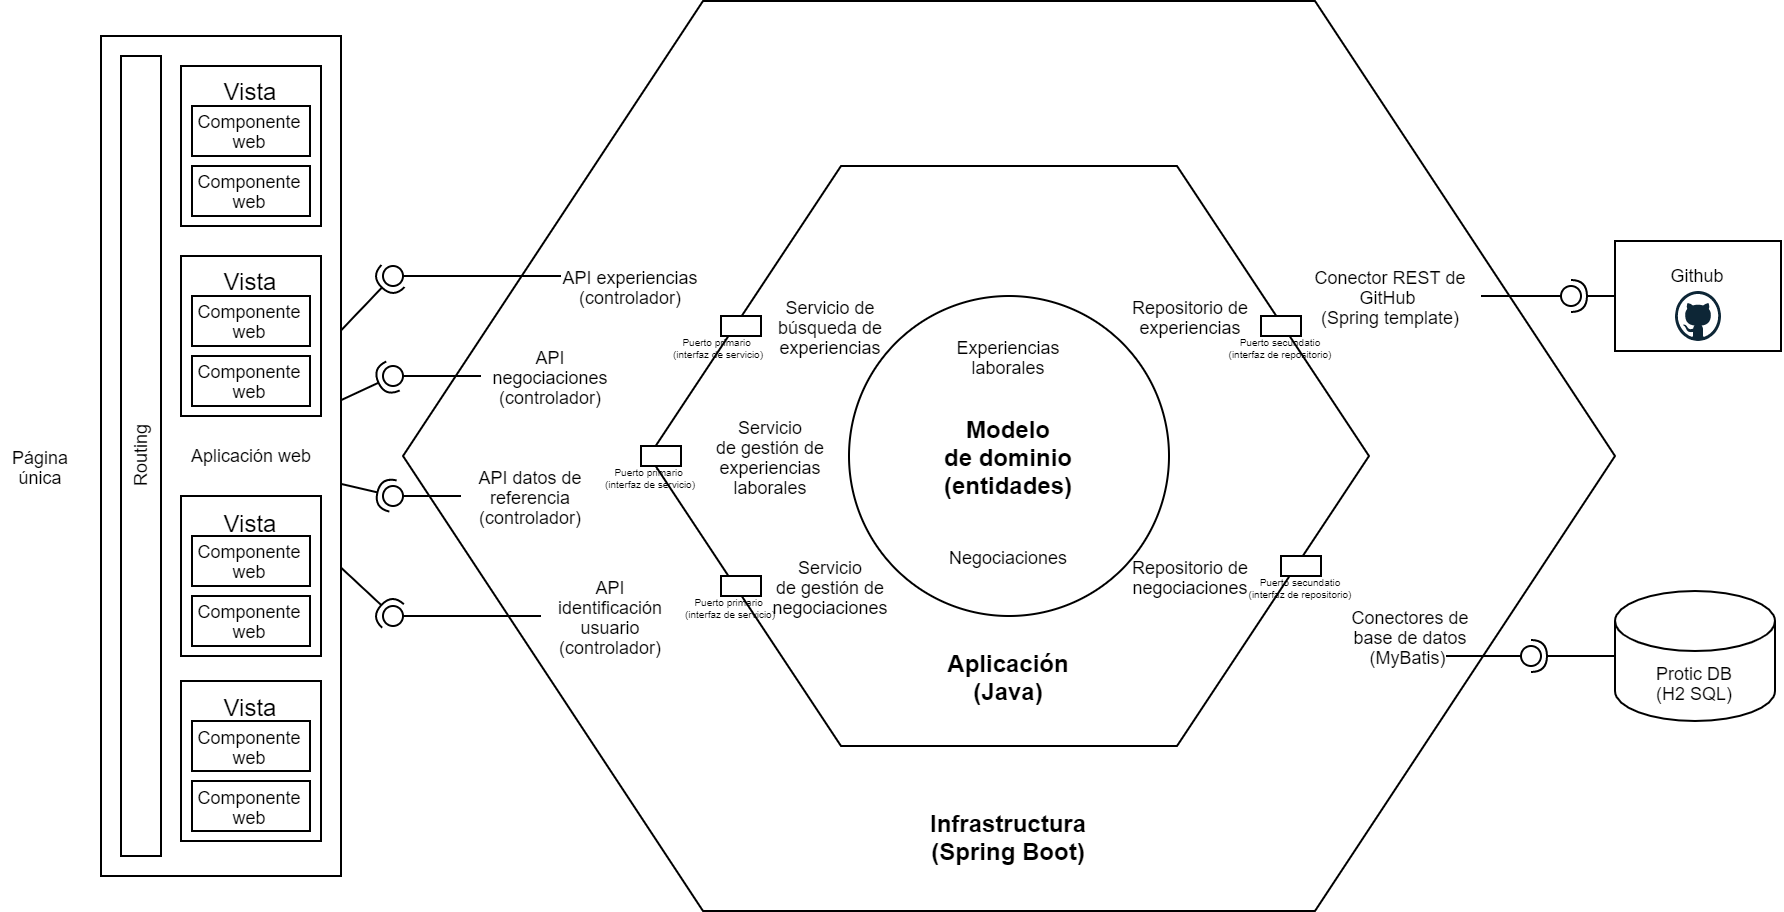
\includegraphics[width=15cm, keepaspectratio]{img/Arquitectura_hexagonal.png}
  \caption{Esquema de la arquitectura general.}\label{fig:general_architecture}
\end{figure}


Por ejemplo, puedes verlo en la figura~\ref{fig:arquitectura}.
\LaTeX \ pone las figuras donde mejor cuadran. 
Y eso quiere decir que quizás no lo haga donde lo hemos puesto\ldots
Eso no es malo.
A veces queda un poco raro, pero es la filosofía de \LaTeX: tú al contenido, que yo me encargo de la maquetación.

\begin{figure}
  \centering
  \includegraphics[width=9cm, keepaspectratio]{img/arquitectura.png}
  \caption{Estructura del parser básico.}\label{fig:arquitectura}
\end{figure}

\begin{figure}
    \centering
    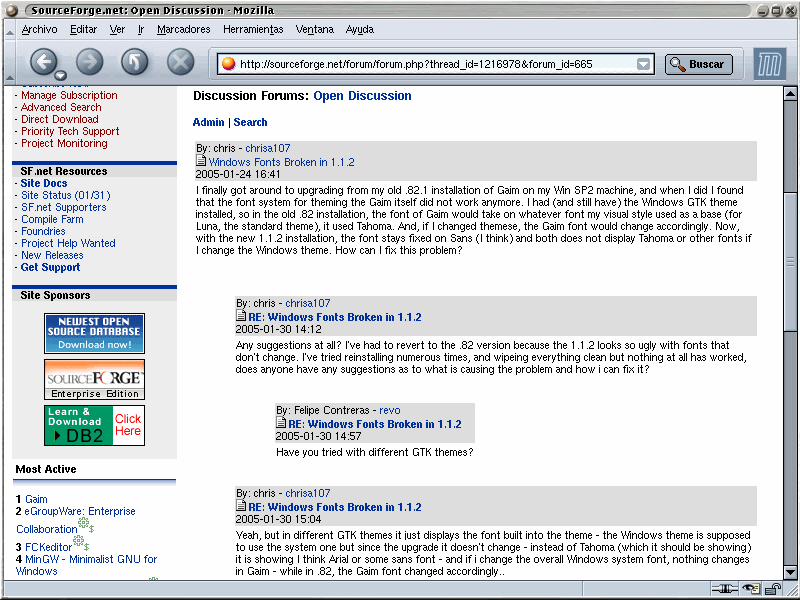
\includegraphics[bb=0 0 800 600, width=12cm, keepaspectratio]{img/foro1}
    \caption{Página con enlaces a hilos}\label{fig:_arquitectura}
\end{figure}

 
Recuerda que toda figura que añadas a tu memoria debe ser explicada.
Sí, aunque te parezca evidente lo que se ve en la figura~\ref{fig:arquitectura}, la figura en sí solamente es un apoyo a tu texto.
Así que explica lo que se ve en la figura, haciendo referencia a la misma tal y como ves aquí.
Por ejemplo: En la figura~\ref{fig:arquitectura} se puede ver que la estructura del \emph{parser} básico, que consta de seis componentes diferentes: los datos se obtienen de la red, y según el tipo de dato, se pasará a un \emph{parser} específico y bla, bla, bla\ldots

Si utilizas una base de datos, no te olvides de incluir también un diagrama de entidad-relación.


%%%%%%%%%%%%%%%%%%%%%%%%%%%%%%%%%%%%%%%%%%%%%%%%%%%%%%%%%%%%%%%%%%%%%%%%%%%%%%%%
%%%%%%%%%%%%%%%%%%%%%%%%%%%%%%%%%%%%%%%%%%%%%%%%%%%%%%%%%%%%%%%%%%%%%%%%%%%%%%%%
% EXPERIMENTOS Y VALIDACIÓN %
%%%%%%%%%%%%%%%%%%%%%%%%%%%%%%%%%%%%%%%%%%%%%%%%%%%%%%%%%%%%%%%%%%%%%%%%%%%%%%%%

\cleardoublepage
\chapter{Experimentos y validación}

Este capítulo se introdujo como requisito en 2019. 
Describe los experimentos y casos de test que tuviste que implementar para validar tus resultados. 
Incluye también los resultados de validación que permiten afirmar que tus resultados son correctos. 


%%%%%%%%%%%%%%%%%%%%%%%%%%%%%%%%%%%%%%%%%%%%%%%%%%%%%%%%%%%%%%%%%%%%%%%%%%%%%%%%
%%%%%%%%%%%%%%%%%%%%%%%%%%%%%%%%%%%%%%%%%%%%%%%%%%%%%%%%%%%%%%%%%%%%%%%%%%%%%%%%
% RESULTADOS %
%%%%%%%%%%%%%%%%%%%%%%%%%%%%%%%%%%%%%%%%%%%%%%%%%%%%%%%%%%%%%%%%%%%%%%%%%%%%%%%%

\cleardoublepage
\chapter{Resultados}

En este capítulo se incluyen los resultados de tu trabajo fin de grado.

Si es una herramienta de análisis lo que has realizado, aquí puedes poner ejemplos de haberla utilizado para que se vea su utilidad.


%%%%%%%%%%%%%%%%%%%%%%%%%%%%%%%%%%%%%%%%%%%%%%%%%%%%%%%%%%%%%%%%%%%%%%%%%%%%%%%%
%%%%%%%%%%%%%%%%%%%%%%%%%%%%%%%%%%%%%%%%%%%%%%%%%%%%%%%%%%%%%%%%%%%%%%%%%%%%%%%%
% CONCLUSIONES %
%%%%%%%%%%%%%%%%%%%%%%%%%%%%%%%%%%%%%%%%%%%%%%%%%%%%%%%%%%%%%%%%%%%%%%%%%%%%%%%%

\cleardoublepage
\chapter{Conclusiones}
\label{chap:conclusiones}


\section{Consecución de objetivos}
\label{sec:consecucion-objetivos}

Esta sección es la sección espejo de las dos primeras del capítulo de objetivos, donde se planteaba el objetivo general y se elaboraban los específicos.

Es aquí donde hay que debatir qué se ha conseguido y qué no. 
Cuando algo no se ha conseguido, se ha de justificar, en términos de qué problemas se han encontrado y qué medidas se han tomado para mitigar esos problemas.

Y si has llegado hasta aquí, siempre es bueno pasarle el corrector ortográfico, que las erratas quedan fatal en la memoria final.
Para eso, en Linux tenemos aspell, que se ejecuta de la siguiente manera desde la línea de \emph{shell}:

\begin{verbatim}
  aspell --lang=es_ES -c memoria.tex
\end{verbatim}

\section{Aplicación de lo aprendido}
\label{sec:aplicacion}

Aquí viene lo que has aprendido durante el Grado/Máster y que has aplicado en el TFG/TFM. Una buena idea es poner las asignaturas más relacionadas y comentar en un párrafo los conocimientos y habilidades puestos en práctica.

\begin{enumerate}
  \item a
  \item b
\end{enumerate}


\section{Lecciones aprendidas}
\label{sec:lecciones_aprendidas}

Aquí viene lo que has aprendido en el Trabajo Fin de Grado/Máster.

\begin{enumerate}
  \item Aquí viene uno.
  \item Aquí viene otro.
\end{enumerate}


\section{Trabajos futuros}
\label{sec:trabajos_futuros}

Ningún proyecto ni software se termina, así que aquí vienen ideas y funcionalidades que estaría bien tener implementadas en el futuro.

Es un apartado que sirve para dar ideas de cara a futuros TFGs/TFMs.


%%%%%%%%%%%%%%%%%%%%%%%%%%%%%%%%%%%%%%%%%%%%%%%%%%%%%%%%%%%%%%%%%%%%%%%%%%%%%%%%
%%%%%%%%%%%%%%%%%%%%%%%%%%%%%%%%%%%%%%%%%%%%%%%%%%%%%%%%%%%%%%%%%%%%%%%%%%%%%%%%
% APÉNDICE(S) %
%%%%%%%%%%%%%%%%%%%%%%%%%%%%%%%%%%%%%%%%%%%%%%%%%%%%%%%%%%%%%%%%%%%%%%%%%%%%%%%%

\cleardoublepage
\appendix
\chapter{Manual de usuario}
\label{app:manual}

Esto es un apéndice.
Si has creado una aplicación, siempre viene bien tener un manual de usuario.
Pues ponlo aquí.

%%%%%%%%%%%%%%%%%%%%%%%%%%%%%%%%%%%%%%%%%%%%%%%%%%%%%%%%%%%%%%%%%%%%%%%%%%%%%%%%
%%%%%%%%%%%%%%%%%%%%%%%%%%%%%%%%%%%%%%%%%%%%%%%%%%%%%%%%%%%%%%%%%%%%%%%%%%%%%%%%
% BIBLIOGRAFIA %
%%%%%%%%%%%%%%%%%%%%%%%%%%%%%%%%%%%%%%%%%%%%%%%%%%%%%%%%%%%%%%%%%%%%%%%%%%%%%%%%

\cleardoublepage

% Las siguientes dos instrucciones es todo lo que necesitas
% para incluir las citas en la memoria
\bibliographystyle{abbrv}
\bibliography{memoria}  % memoria.bib es el nombre del fichero que contiene
% las referencias bibliográficas. Abre ese fichero y mira el formato que tiene,
% que se conoce como BibTeX. Hay muchos sitios que exportan referencias en
% formato BibTeX. Prueba a buscar en http://scholar.google.com por referencias
% y verás que lo puedes hacer de manera sencilla.
% Más información: 
% http://texblog.org/2014/04/22/using-google-scholar-to-download-bibtex-citations/

\end{document}
